% !TeX spellcheck = en_US
\documentclass[a4paper]{article}
\usepackage[utf8]{inputenc}
\usepackage{t1enc}
\usepackage[english]{babel}
\usepackage{lmodern}
\usepackage{url}
\usepackage{graphics}
\usepackage{listings}
\usepackage[a4paper, total={5.4in, 8in}]{geometry}

\hyphenation{UPPAAL}
\sloppy

\begin{document}
	
	\newcommand{\specialcell}[2][c]{%
		\begin{tabular}[#1]{@{}c@{}}#2\end{tabular}}
	
	\newenvironment*{mytable}[3]{
		% #1: caption, #2: cimke, #3: oszlopdef		 
		\begin{table}[htbp]	
			\caption{#1}          
			\label{tab:#2}            
			\center%
			\begin{tabular}{#3}
			}
			{
			\end{tabular}
		\end{table}
	}
	
	\pagestyle{plain}
	
	
	
	% angol környezet beállítása
	\nonfrenchspacing
	\setlength{\parindent}{0em}
	\setlength{\parskip}{0.45em}
	
	\title{Language Learning Application: \\ Requirement Specification \\ \begin{large}Software Architectures Homework \end{large}}
	\author{Bence Graics \and Kristóf Verbőczy}	
	\date{}
	\maketitle
	\section*{Introduction}
	This document presents the requirement specification of the software architectures homework \textsl{Language Learning Application}. First, the assigned task is introduced, which is followed by the detailed description of the task. Next, the technical parameters of the software addressing the task is presented. Finally, a use-case diagram is given that depicts the essential use-cases of the software.
	\section{The task}
	The task is to create an application aiding foreign language learning. The foreign words and sentences can be organized into lessons by means of associated meta information. A central server is responsible for the management and storage of data. In addition to a server component, the application comprises of a client component supporting the management of the server as well as the conduction of lessons. The platforms, serving as the basis of the application, can be chosen freely.
	
	\section{Detailed task description}
	
	\section{Technical parameters}
	Java, JavaFx, Maven, REST, Internet
	
	\section{Use-cases}
	\begin{figure}[htbp]
		\center
		\resizebox{135mm}{!} {
			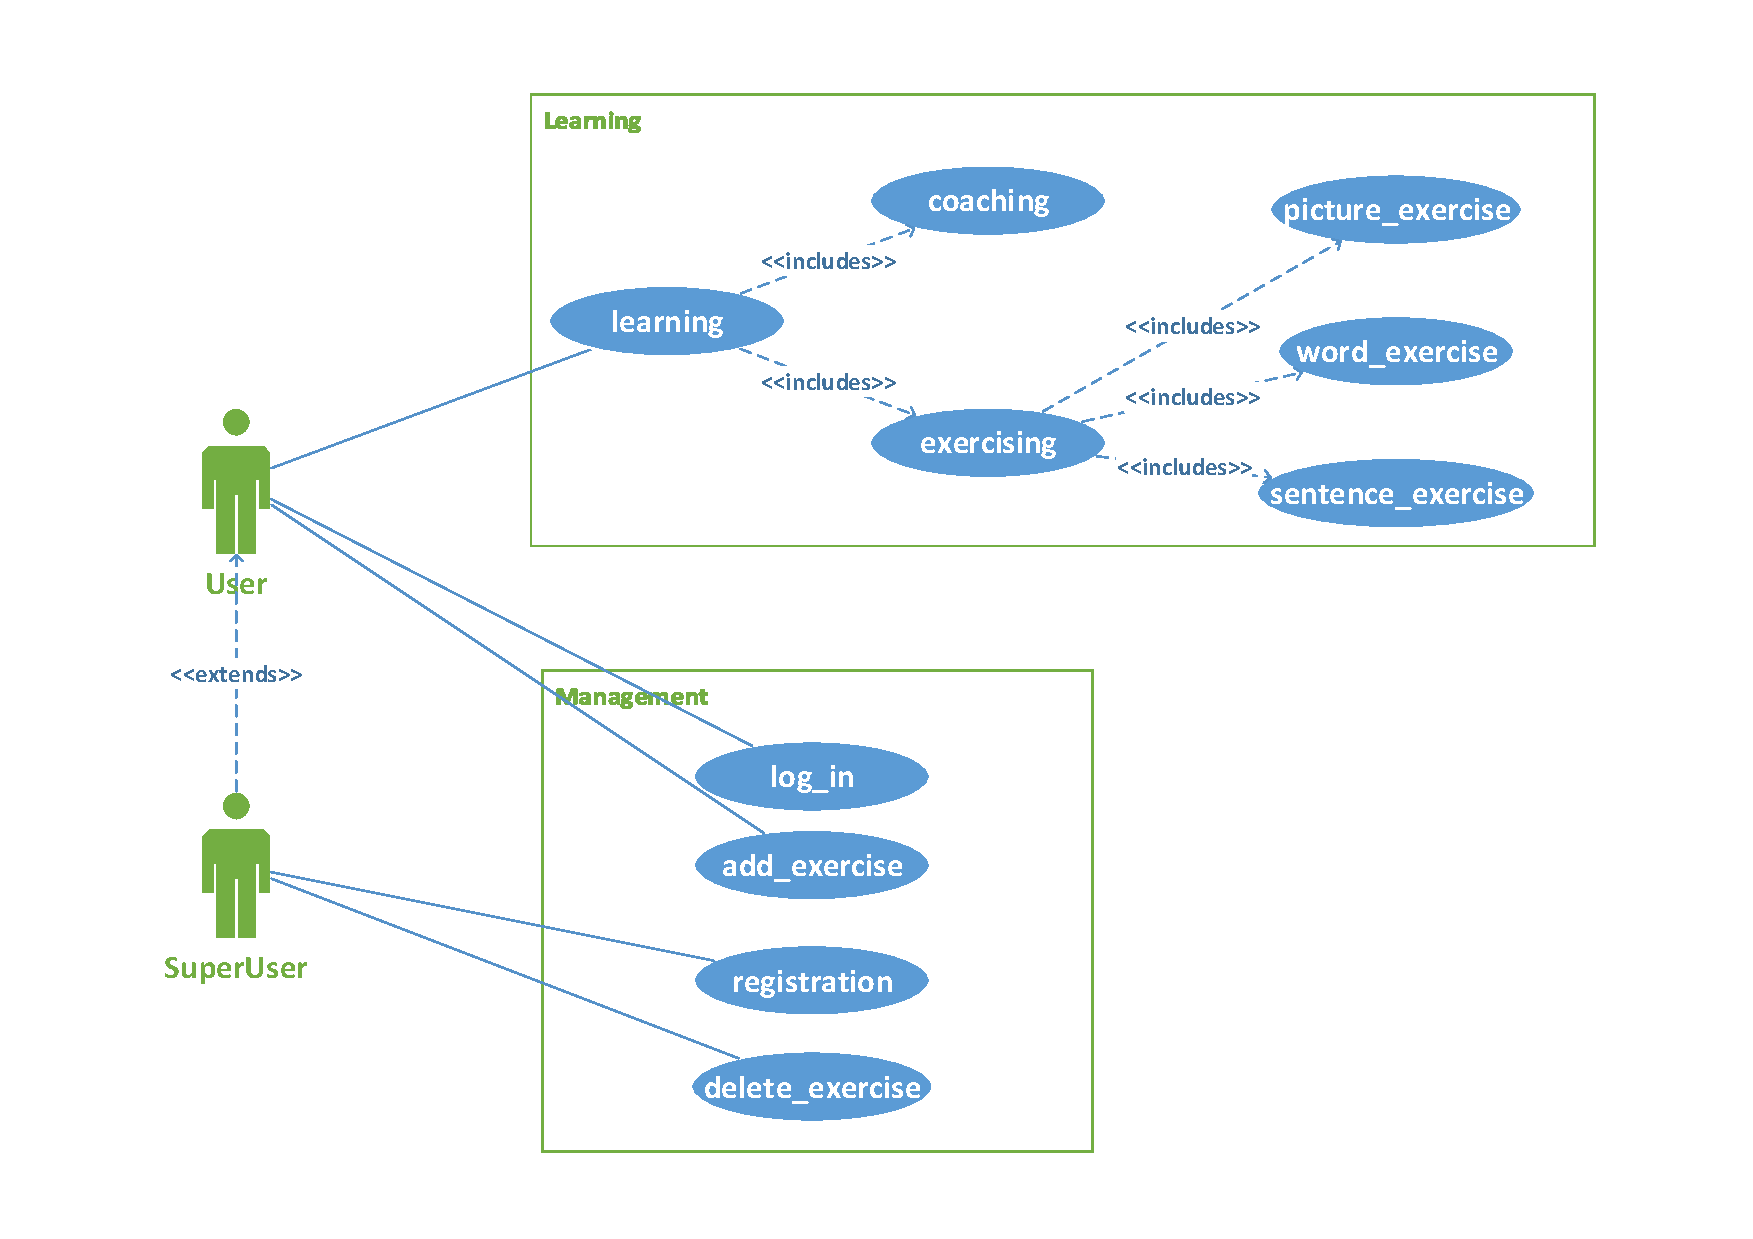
\includegraphics{figures/use-case.pdf}
		}
		\caption{Use-case diagram}
		\label{fig:use-case}
	\end{figure}
%	This tutorial presents the \framework\ from a practical aspect. First, a short summary of the framework functionalities is given which is followed by the presentation of composite system elements as well as the semantics a composite system conforms to. Next, an installation guide setting up the \framework\ is presented. Finally, the functionalities of the framework are demonstrated based on a case-study called MoDeS$^3$.

%	\begin{figure}[htbp]
%		\center
%		\resizebox{135mm}{!}{
%			\includegraphics{fig/gui_window.png}
%		}
%		\caption{The window supporting the verification and back-annotation functionalities of the framework.}
%		\label{fig:gui_window}
%	\end{figure}	
	

\end{document}